




%----------------------------------------------------------------------
\section{Solution Framework}
%----------------------------------------------------------------------

Our solution framework (Figure \ref{Solution framework}) contains two major parts. ``Materialization Part'' takes previous workload as input and perform materialization. We first partition previous queries into ``hot'' queries and ``less hot'' queries based on frequency count of their structures. CubePlanner and StructurePlanner take ``hot'' queries and ``less hot'' queries as input and select cuboids and substructures (in form of tables) for materialization respectively. Subsection \ref{Overview of Materialization Part} will explain intuition of categorization of ``hot'' and ``less hot'' queries and why we pass them to different ``planners''.  ``Future Query Processing Part'' takes future queries as input and generate results. If a future query is of ``hot'' structure we consult cuboid materializations to see if it can be directly answered by aggregation over a cuboid materialization. In this scenario cuboid materialization will be used. If the future query cannot be directly answered by any cuboid materialization, we turn to substructure materializations. We decompose the query into substructures and produce results by ``joining'' these substructures. In this scenario, substructure materializations will be used. 

We will discuss ``Materialization Part'' in Section \ref{Materialization Part} and ``Future Query Processing Part'' in Section \ref{Future Query Processing Part}.

\begin {figure}[H]
\centering
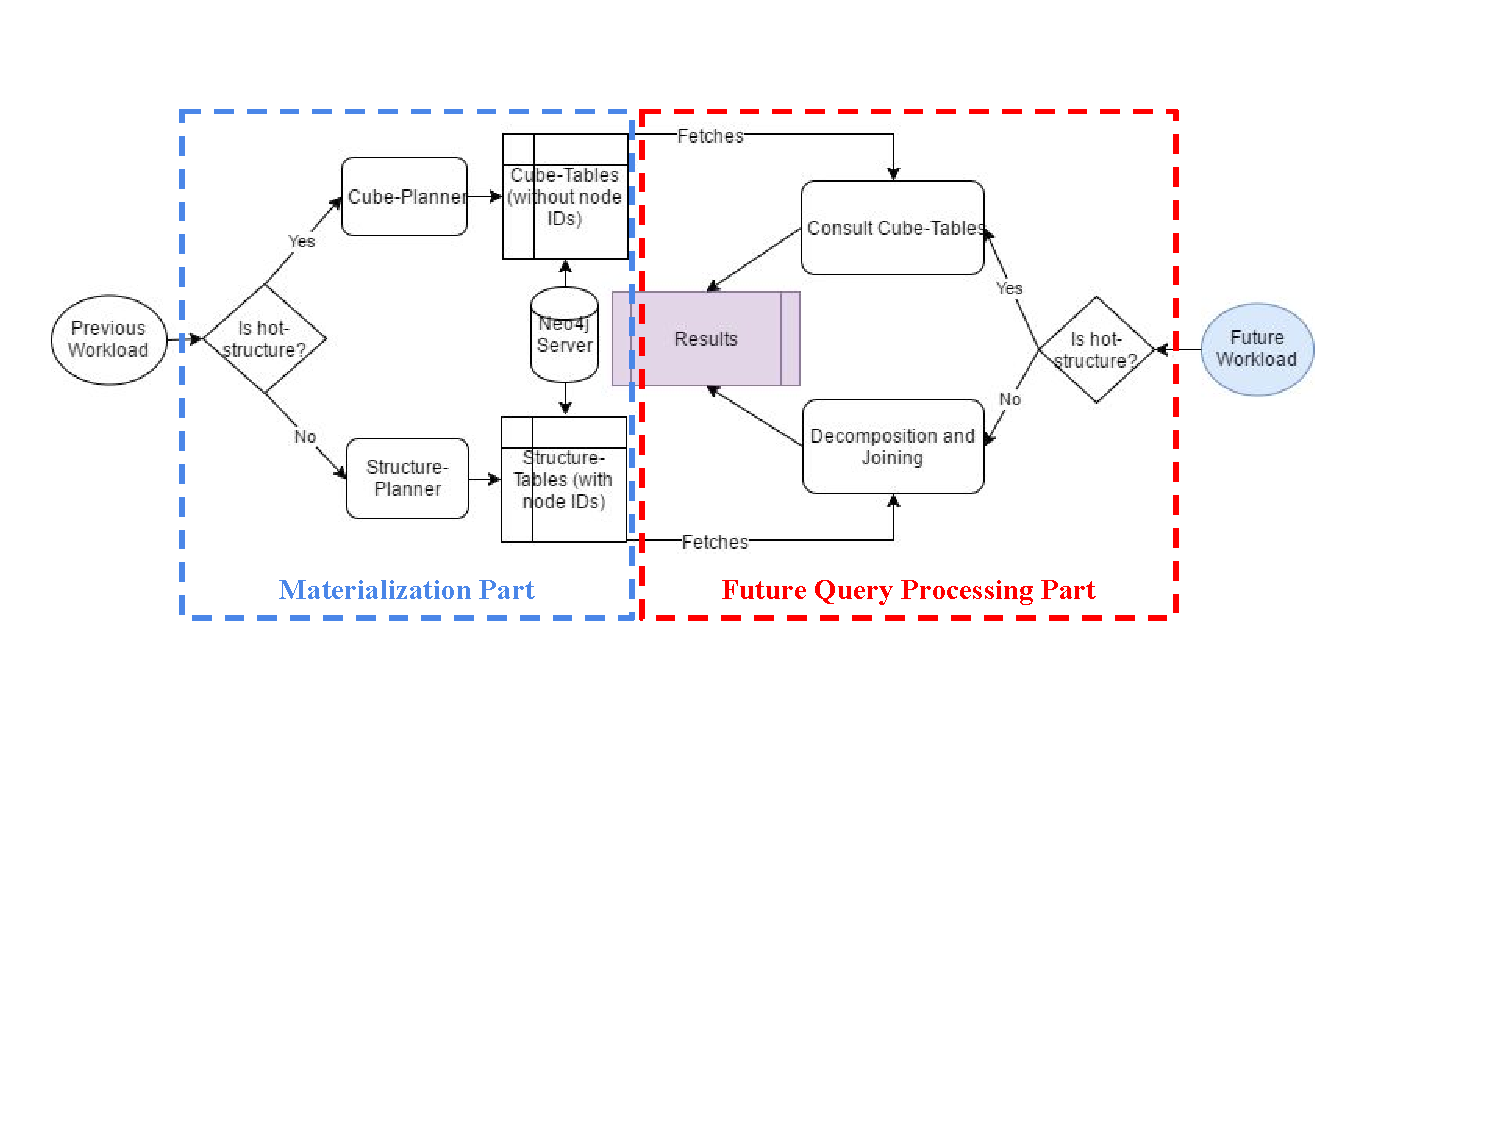
\includegraphics[scale=0.8]{pic/41.pdf}
\caption{Solution framework.}
\label{Solution framework}
\end{figure}


%----------------------------------------------------------------------
\section{Materialized View Selection}
\label{Materialization Part}
%----------------------------------------------------------------------
We will discuss materialized view selection in this section. We will first give an overview of materialized view selection and then focus on cuboid and substructure selections respectively.
%----------------------------------------------------------------------
\subsection{Overview of Materialized View Selection}
\label{Overview of Materialization Part}
%----------------------------------------------------------------------
In Section \ref{Materialization: Cuboid vs Substructures}, we have discussed about the trade-off between cuboids and substructures. We know that utilization of a cuboid materialization requires future queries to have exactly the same structure as the cuboid. It is wise that we materialize a cuboid only when we are confident that the structure of a cuboid is likely to be ``hit'' by future queries, because otherwise we may risk wasting space only to materialize cuboids that are rarely ``hit''. Compared with cuboids, substructures do not have such strict ``structure match'' requirement. A substructure can be used as long as it is covered by a future query. 

We make our materialization policy based on such different features of cuboids and substructures. 
We first perform frequency count of previous queries. For queries of structure frequency over a threshold $\sigma$, consider these queries have ``hot structure'' and pass them to CubePlanner for cuboid selection. For the rest queries with "less hot structure", pass them to StructurePlanner for substructure selection. 

\begin{algorithm}[H]
\caption{Materialization Overview}
\LinesNumbered
\textbf{System setting:} $\sigma$: frequency threshold for hot structures\\ 
\KwIn{Q: a set of previous queries\\}
\KwOut{C: a set of materialized cuboids\\ S: a set of materialized substructures}

$CInput \gets \emptyset$\;
$SInput \gets \emptyset$\;
\ForEach{q \in Q}{
	\eIf{structureFreq(Q, q) $>$ \sigma}{
		$CInput \gets CInput \cup \{q\} $\;
	}{	
		$SInput \gets SInput \cup \{q\} $\;
	}
}
$C:=materialize(CubePlanner(CInput))$\;
$S:=materialize(StructurePlanner(SInput))$\;
\label{alg:PartialMaterialization}
\end{algorithm}
\clearpage

Function $structureFreq(Q, q)$ returns frequency count of $q$'s structure in $Q$. Functions $CubePlanner$ and $StructurePlanner$  return selected cuboids and substructures by CubePlanner and StructurePlanner. Function $materialize$ performs materialization of cuboids and substructures.

For example, suppose we have the following previous queries and future queries.

\textbf{Previous Workload:}

\begin{itemize}
\item \#1 Badge-User, User-Post:Badge.Name,Post.Score,Post.PostTypeId=2

\item \#2 User-Comment, Comment-Post: User.UpVotes, Comment.Score, (AVG)Post.Score, Post.PostTypeId=1

\item \#3 User-Post, Post-Vote: User.UpVotes, Vote.VoteTypeId

\item \#4 User-Post, Post-Tag: (AVG)User.CreationDate\_Year, Tag.TagName

\item \#5 User-Comment, Comment-Post: User.ActiveMonth, Post.CreationDate\_Year=2016

\item \#6 User-Comment, Comment-Post: User.Age, (AVG)Comment.Score, Post.PostTypeId=2
\end{itemize}


\\
\textbf{Future Workload:}

\begin{itemize}
\item \#1 User-Comment, Comment-Post: User.UpVotes, (AVG)Post.Score, Post.PostTypeId

\item \#2 User-Comment, Comment-Post: User.Age, Post.PostTypeId

\item \#3 User-Post, Post-PostHistory: User.UpVotes, PostHistory.PostHistoryTypeId

\item \#4 Badge-User, User-Post:(AVG)Post.Score,Post.PostTypeId=2
\end{itemize}

\par
We count previous queries by structure:

\begin{center}
\begin{tabular}{ | c | c |}  
	\hline
	Structure	&Frequency	\\ \hline 
	\textbf{User-Comment, Comment-Post} 	&\textbf{3} \\ \hline
	User-Post, Post-Tag 	&1 \\ \hline
	User-Post, Post-Vote	&1 \\ \hline
\end{tabular}
\end {center}
\par	
We are confident that \textit{User-Comment, Comment-Post} is a ``hot structure''. We materialize cuboids over structure \textit{User-Comment, Comment-Post} by passing previous query \#2, \#5 and \#6 to CubePlanner. CubePlanner will materialize cuboids that benefit processing of future query \#1 and \#2 (which have \textit{User-Comment, Comment-Post} structure).
\par
We pass the three remaining queries of ``less hot structure'' previous query \#1, \#3 and \#4 to StructurePlanner. StructurePlanner will discover and materialize most useful substructures. In this case StructurePlanner is likely to find \textit{User-Post} as a useful substructure it can be used in joining the result of future query \#3 and \#4.
%----------------------------------------------------------------------
\subsection{Greedy Selection Framework}
%----------------------------------------------------------------------

We adopt a greedy selection framework in materialized view selection. In our solution framework, CubePlanner and StructurePlanner are responsible for materialized view selection (over cuboids and substructures respectively). They both adopt the same greedy selection framework. In Section \ref{sec:Problem Definition}, we introduced that ``Materialization Selection Problem'' aims at finding best materializations under a space limit $\sigma$. ``Materialization Selection Problem'' is known to be an NP-hard problem \cite{DBLP:journals/kais/LinK04}. It is hard because overall benefit of materialized views is not a simple sum of individual benefit of each materialized view. A materialized view's marginal benefit may be deducted when another view is selected. For example, marginal benefit of a substructure over ``\textit{User-Post, Post-Tag}'' will be affected by selection of substructures over ``\textit{User-Post}'' and ``\textit{Post-Tag}''. A naive approach to solve ``Materialization Selection Problem'' is to enumerate over all possible combinations of cuboids $C$ and substructures $S$ within the space limit $\sigma$ and find the best combination. But such naive may results in an unacceptable time complexity. What's worse, suppose we find an answer $C'$ and $S'$ in a naive way. It is not guaranteed that actual total space cost of $C'$ and $S'$ is strictly lower than $\sigma$ as we made estimations in our calculation. As a result, we turn to a greedy algorithm which is better than naive approach in terms of efficiency, besides it allows materializations to be done one by one until space limit $\sigma$ is hit.

We will discuss this greedy selection framework first so that readers have a high-level idea of our selection policy. We use greedy algorithms for cuboid and substructure selection. The idea is to always pick next candidate with highest ratio of margin benefit against space. After a candidate is picked, we re-evaluate benefit of remaining candidates. Re-evaluation is essential as margin benefit of a candidate may be deducted owing to materialization of a selected candidate. 


\begin{algorithm}[H]
	\caption{Greedy Selection}
	\LinesNumbered  
	\textbf{System setting:} $\sigma$: space limit\\ 
	\KwIn{C: a set of candidates of cuboids or substructures in lattice structure\\ P: A set of previous queries}
	\KwOut{Q: a queue of selected candidates to materialize\\ }
	\ForEach{c \in C}{
		c.space := space(c)\;
		c.benefit := estimateMarginBenefit(c, P, Q)\;
		c.score := c.benefit/c.space\;
	} 
	
	\While{$Q.totalsize < \sigma$}{
		selected := c in C with highest score\;  
		Q.Enqueue(selected)\;
		repeat Lines 1-5\;
	}
\end{algorithm}

We use a queue as data structure for output $Q$ in above algorithm presentation because in some cases we may want to keep information of orders of selection. When selection orders are not important we may as well simply use a set to store selected views. Line 1-5 estimates space cost, marginal benefit for future workload, and score for each candidate. We call this parse  \textbf{``score calculation''}. Line 6-10 keeps picking up candidates with highest score one by one until space limit is hit. Notice that each time a candidate is selected, Line 9 refreshes scores for all candidates by repeating 1-5. We call this parse \textbf{``pick-and-update''}.   

CubePlanner and StructurePlanner apply this greedy selection framework by implementation of ``score calculation'' and ``pick-and-update''. Future users can vary CubePlanner and StructurePlanner by plug-ins of their own implementation with consideration of their database features. We will introduce how we implement our CubePlanner and StructurePlanner for Neo4j in the following subsections.

%----------------------------------------------------------------------
\subsection{CubePlanner}
%----------------------------------------------------------------------  

We will discuss CubePlanner in this section. CubePlanner takes ``hot'' previous queries as input and output selected cuboid materializations. In Subsection \ref{Materialization: Cuboid vs Substructures}, we mentioned that one feature about cuboid is that cuboid are only useful for queries of exactly same structure. To put it another way, cuboids of different structures do not affect each other at all in terms of benefits for future queries. As a result even though input queries for CubePlanner may have different structures, we can group queries by structure and treat them individually. For each group of input queries we propose algorithm ``SingleCubePlanner'' to select top-$n$ cuboids. After all groups are finished, we select final results across top-$n$ cuboids of all groups. A good analogy for such process is to first hold regional competitions and then select national winners from regional winners. We will discuss algorithm ``CubePlanner'' in Subsection \ref{CubePlanner}, followed by ``SingleCubePlanner'' explained in Subsection \ref{SingleCubePlanner}.

%----------------------------------------------------------------------
\subsubsection{CubePlanner}
\label{CubePlanner}
%---------------------------------------------------------------------- 

As we mentioned above, CubePlanner performs cuboid selection in a holistic manner by one-by-one selection of cuboids from results of SingleCubePlanners. 

\begin{algorithm}[H]
	\caption{CubePlanner}
	\LinesNumbered 
	\textbf{System setting:} 
	: maximum number of cuboids to precompute\\ 
	\KwIn{Q: a set of previous queries not nessesarily with a same structure}
	\KwOut{C: a queue of selected cuboids to precompute\\ }
	Group:= group(Q)\;
	\ForEach{group \in Group}{
		group.results := SingleCubePlanner(group);
	} 
	
	\For{i=1 \emph{\KwTo} n}{
		group' := group in Group with highest group.results.top().score\; 
		C.offer(group'.Dequeue())\;
	}
	
\end{algorithm}
\clearpage

Function $group(Q)$ groups $Q$ by structure. $SingleCubePlanner$ will be discussed in Subsection \ref{SingleCubePlanner}. 

Line 1 partitions $Q$ by structure. Each partition consists of previous queries of a same structure, which will be passed to a SingleCubePlanner. Line 2-4 performs cuboid selection in each partition using SingleCubePlanner. An ordered queue of candidates is generated by each SingleCubePlanner. Line 5-8 repeatedly checks current top candidate for each partition and picks out the best candidate among them. $n$ is a user defined parameter. In our implementation select $n$ at most cuboids for materialization.  Users may choose other ways such as a space limit as a bound for cuboid materiliazation.

%----------------------------------------------------------------------
\subsubsection{SingleCubePlanner}
\label{SingleCubePlanner}
%----------------------------------------------------------------------  

Given previous queries of a same structure, we implement algorithm ``SingleCubePlanner'' from greedy selection framework to select top-$n$ cuboids. 

\begin{algorithm}[H]
	\caption{SingleCubePlanner}
	\LinesNumbered 
	\textbf{System setting:} n: as in ``top-$n$''\\ 
	\KwIn{P: a set of previous queries with a same structure}
	\KwOut{C: an queue of selected cuboids to precompute\\ }
	$Lattice \leftarrow buildLattice(Q)$\;
	\ForEach{query $Q$ \in P}{
		$q.time \leftarrow time(q)$\;
	} 
	\ForEach{cuboid \in Lattice}{
		$cuboid.space \leftarrow space(cuboid) $\;
		$cuboid.benefit \leftarrow 0$\;
		\ForEach{query $Q$ $\in$ $P$ and q.properties $\subseteq$ cuboid.properties}{
			$cuboid.benefit +=max(0, q.time-aggreTime(cuboid))$\;
		}
		$cuboid.score \leftarrow cuboid.benefit/cuboid.space$\;
	}
	\For{i=1 \emph{\KwTo} n}{
		nextBestCube $\gets$ cuboid in Lattice with highest score\;
		\If{$nextBestCube.score < 0$}{
			break\;
		}
		C.Enqueue(nextBestCube)\;
		\ForEach{cuboid $Q$ $\in$ $Q$ and q.dimension $\subseteq$ nextBestCube.dimension }{
			$q.time \gets min(q.time, aggreTime(nextBestCube)) $\;
		}
		repeat 5-12\;
	}
	
\end{algorithm}
\clearpage

Line 1 builds a lattice over all combinations of dimensions of all attributes which appeared in previous queries $P$ using classic lattice construction algorithms \cite{DBLP:journals/ipl/NourineR99}. Line 2-4 initializes best-so-far processing time for each previous query by its estimated naive database processing time. Line 5-12 performs ``score calculation'' in ``greedy selection framework''. For each cuboid, Line 6 estimates its space. Line 8-10 calculates marginal benefit. Line 8 iterates over previous queries that can be answered by scanning current cuboid. If estimated scanning time is less than a previous query's current best-so-far processing time, we add the difference of two times to the cuboid's total marginal benefit (Line 9). Line 13-23 performs ``pick-and-update'' in ``greedy selection framework''. Line 15-17 terminates selection when there is no extra marginal benefit any more. Line 19-22 updates best-so-far processing time for previous queries as a result of current round of selection.

Implementation of functions are listed as follows. Notice that users can implement these functions in their own ways based on their database systems. Function \textbf{$time(query)$} estimates naive time cost for processing a query by a graph database. Implementation of $time(query)$ is database specific as physical storage and execution plans vary among different databases. Since Neo4j provide APIs to see execution plan and estimated intermediate result size, we directly use total size of intermediate results as an estimation of time cost. For example, Figure \ref{fig:4:2} is an execution plan provided by Neo4j for query \textit{User-Badge, User-Post, Post-Tag: Tag.TagName}. We can see that numbers of ``estimated rows'' for intermediate results are provided. We use  $\displaystyle{\sum ``estimated\_rows''}$ to estimate total processing time cost.

\begin {figure}[H]
\centering
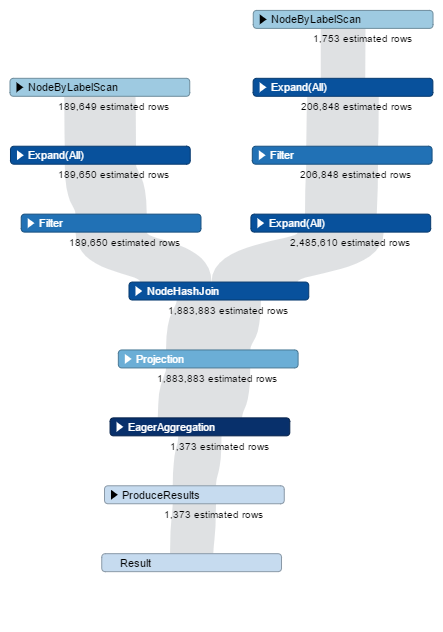
\includegraphics[scale=0.6]{pic/61.png}
\caption{Neo4j's execution plan for query \textit{User-Badge, User-Post, Post-Tag: Tag.TagName}.}
\label{fig:4:2}
\end{figure}

For graph databases where such APIs to see  execution plans and estimated intermediate result sizes are not provided, users need to provide estimation based on their understanding about the database. There are many studies on cost estimations for database operations (joins etc). Users may consider joining (expanding) order \cite{DBLP:conf/pods/Chaudhuri98} and estimation of intermediate result sizes  \cite{DBLP:conf/edbt/SwamiS94} as two important aspects. 

Function \textbf{$aggreTime(cuboid)$} estimates time cost for a scanning cuboid materialization. For cuboid $c$, we use space cost of $c$ for estimation. 

$spacePerRow:= 
\displaystyle{\sum_{p\in c.properties}sizeOf(p)}$

$SpaceCost(c):= spacePerRow *  numberOfRows(c)$

Here \textit{sizeOf(property type)} refers to standard size of data types. For exmaple integer type in ``C++'' is 2 byte. \textit{numberOfRows(c)} refers to number of rows of $c$. A rough estimation is the product of cardinalities of all queried properties. 

$numberOfRows(c):= \displaystyle{\prod_{p\in c.properties}|p|} $


%----------------------------------------------------------------------
\subsection{Structure Planner}
\label{Structure Planner}
%----------------------------------------------------------------------
Like CubePlanner, Structure Planner also adopts greedy selection framework.

\begin{algorithm}[H]
\caption{StructurePlanner}
\LinesNumbered 
\textbf{System setting:} n: maximum number of substructures to precompute\\ 
\KwIn{Q: a set of previous queries}
\KwOut{S: an queue of selected substructures to precompute\\ }
$Lattice \leftarrow buildSubstuctureLattice(Q)$\;
\ForEach{q \in Q}{
	$q.coveredSubstructres:= \emptyset $\;
} 
\ForEach{substructure \in Lattice}{
	$substructure.space \leftarrow space(substructure) $\;
	$substructure.benefit \leftarrow 0$\;
	\ForEach{q $\in$ $Q$ and q.structure $\subseteq$ substructure.structure}{
		$cuboid.benefit +=max(0, benefit(q, substructure, q.coveredSubstructres))$\;
	}
	$substructure.score \leftarrow substructure.benefit/substructure.space$\;
}
\For{i=1 \emph{\KwTo} n}{
	nextBestSubstructre $\gets$ substructure in Lattice with highest substructure.score\;
	\If{$nextBestSubstructre.score < 0$}{
		break\;
	}
	S.offer(nextBestSubstructre)\;
	\ForEach{q $\in$ $Q$ and q.structure $\subseteq$ nextBestSubstructre.structure }{
		$q.coveredSubstructres \gets q.coveredSubstructres \cup \{nextBestSubstructre \} $\;
	}
	repeat 5-12\;
}

\end{algorithm}
\clearpage

Line 1 builds a lattice over all substructures of previous queries $P$, using classic lattice construction algorithms (similar to lattice construction algorithms in CubePlanner). Figure \ref{fig:4:3} shows a substructure lattice originating from root node \textit{Badge-User, User-Post, Post-Tag}. Starting from a union of structures of previous queries as the root node, a lattice can be constructed recursively by populating descendants from parent nodes through edge removals.

\begin {figure}[H]
\centering
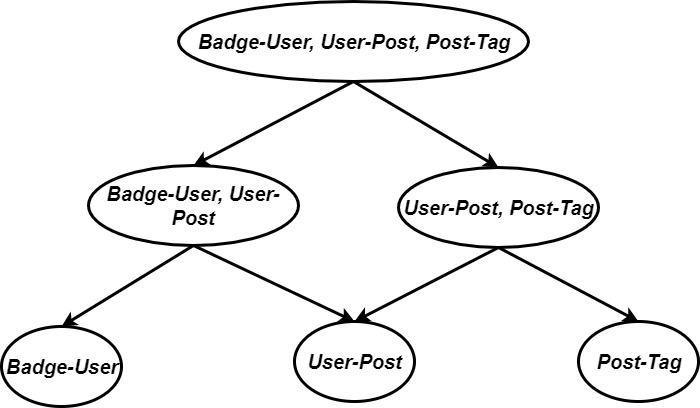
\includegraphics[scale=0.6]{pic/Structurelattice.jpg}
\caption{A substructure lattice with \textit{Badge-User, User-Post, Post-Tag} as its root node.}
\label{fig:4:3}
\end{figure}


Line 2-4 initializes covered substructures for each previous query as empty. For a previous query, $coveredSubstructure$ keeps what substructures have been selected so far which are useful for processing this query. It will be updated each time a new substructure is selected.
Line 5-12 performs ``score calculation'' in ``greedy selection framework''. For each substructure, Line 6 estimates its space. Line 8-10 iterates over all ``favored'' previous queries (favored by current substructure) and adds on marginal benefit (if any). Here marginal benefit refers to the time saved after adding current substructure to selected substructures (Line 9). Line 13-23 performs ``pick-and-update'' in ``greedy selection framework''. Line 15-17 terminates selection when there is no marginal benefit any more. Line 19-22 updates covered substructures for previous queries as a result of current round of selection.

Implementation of functions are listed as follows. Again users can implement these functions in their own ways based on their database systems. Function \textit{space(substructure)} returns estimated space cost of a substructure materialization. We use Neo4j's execution plan API to get estimated result size of a substructure. Function \textit{benefit(q, substructure, q.coveredSubstructres)} evaluates marginal benefit of substructure to query $Q$ when substructures in $q.coveredSubstructres$ have been materialized. We know that execution plan and estimated intermediate result size are provided by Neo4j's API. But such information is on database's naive processing plan. When substructure materialization is used, execution plan (intermediate result) becomes different from naive processing plan. As a result estimation on marginal benefit of a substructure is tricky. We use $time(q.coveredSubstructres \cup substructure)$ - $time(q.coveredSubstructres)$ for estimation of marginal benefit of a substructure. We think that this roughly indicates overall improvement of adding $substructure$ to $coveredSubstructres$ as materializations.



%----------------------------------------------------------------------
\subsection{ID and Property Selection}
%----------------------------------------------------------------------

Given a substructure picked by Structure Planner, we need to decide on which IDs and properties should be stored. Keeping all IDs and attributes makes a substructure materialization more informative but increases space cost. We are faced with a trade-off between space cost and usage potential. Selection on IDs and properties is an important issue. We will use substructure \textit{User-Post, Post-Tag} as an example and discuss different ID and property selection policies.

For IDs, we consider the following two policies.

\begin{itemize}
\item Policy \#1 keeps IDs of all nodes and edges. This enables ``overlap'' join with other substructures but increases space cost. For \textit{User-Post, Post-Tag}, if we keep IDs of all nodes and edges, then we can perform join operation with \textit{Badge-User, User-Post}. We call such join an ``overlap'' join as the two substructures have an overlap part which is \textit{User-Post}. Note that we can join the two substructures only when IDs of nodes (User and Post), and edge (edge between User and Post) are stored in both substructures.

\item Policy \#2 only keeps IDs of ``border nodes'' which are on the border of the substructure's \textit{structure}. Figure \ref{border node} highlights ``border nodes'' of structure \textit{User-Post, Post-Tag}. In this example we only save IDs of User and Tag. We do not keep IDs of Post as node Post is not located on the border of the \textit{structure}. Compared to Policy \#1, this saves space cost but ``overlap join'' with other substructures is not enabled. Policy \#2 only enables joins on border nodes. For example we may join \textit{User-Post, Post-Tag} with \textit{User-Badge} on their common border node User.

\begin{figure}[H]
\centering
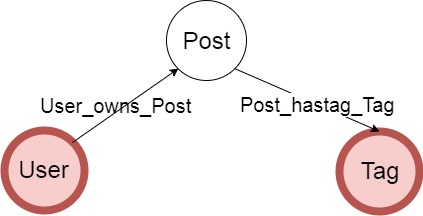
\includegraphics[scale=0.7]{pic/bordernode.jpg}
\caption{``Border nodes'' of structure \textit{User-Post, Post-Tag}.}
\label{border node}
\end{figure}
\end{itemize}


We use Policy \#1 in our implementation. However if keeping IDs of inner nodes and edges overwhelmingly increases result length, it's wise to choose Policy \#2 as space cost becomes too high. 

For properties, we consider the following two policies.

\begin{itemize}
\item Policy \#1 keeps all properties.
\item Policy \#2 only keeps properties that were queried in previous workloads.
\end{itemize}

Our suggestion is to consider the proportion of properties which were queried in previous workload over all properties in the data schema. For example, in our experiment only a small proportion of properties were queried. We choose Policy \#2 as it is a waste of space to keep all properties. 


%----------------------------------------------------------------------
\section{Query Processing}
\label{Future Query Processing Part}
%----------------------------------------------------------------------
Future Query Processing Part aims at processing future queries efficiently using substructure and cuboid materializations. When future query $Q$ arrives, we first consult cuboids materializations. If $Q$ can be answered by aggregation over any cuboid materializations, we select the cuboid with minimum space and directly scan over it to produce result of $q$. If $Q$ cannot be answered by any cuboid, we decompose $Q$ and use substructures to compose the result of $q$. 

\begin{algorithm}[H]
\caption{FutureQueryProcessing}
\LinesNumbered
\textbf{System:} C: a set of materialized cuboids\\ S: a set of materialized substructures\\ 
\KwIn{q: a query\\}
\KwOut{r: result of q}

$minspace:= \infty $\;
mincuboid := NULL\;
\ForEach{$cuboid \in C$}{
\If{cuboid.structure = q.structure and q.dimension \subseteq cuboid.dimension}{
	\If{$cuboid.space<minspace$}{
		minspace := cuboid.space\;
		mincuboid := cuboid\;
	}
}

\eIf{$mincuboid \not= NULL$}{
	$r := aggregate(mincuboid, q)$\;
}{
	$r :=Decompose\_Join(q)$\;
}
}
\end{algorithm}
\clearpage

Line 4-9 looks up materialized cuboids and find if any cuboid can be used to answer query $q$. If there are multiple useful cuboids we use the cuboid with the smallest scanning cost ($cuboid.space$). Note that $cuboid.space$ was computed in Line 9 in Algorithm SingleCubePlanner in Section \ref{SingleCubePlanner}. Line 10 checks if $q$ can be answered by cuboid materializaiton. If yes we perform aggregation operation over the cuboid (Line 11). Otherwise we need to decompose $q$ into substructures and compose the result (Line 13). Function $aggregate(mincuboid, q)$ is classic aggregation operation. We will discuss how function $Decompose\_Join(q)$ is implemented in the following subsections. 

%----------------------------------------------------------------------
\subsection{Substructure Selection}
\label{Substructure Selection}
%----------------------------------------------------------------------

Before discussion on $Decompose\_Join(q)$, we need to first solve a ``Substructure Selection'' problem. In order to decompose a query $q$, we need to consider which materialized substructures we need to use. We need to make dicision when candidate substructures in $S$ overlap. For example suppose $q$ has structure \textit{Badge-User, User-Post, Post-Tag}.

And S consists of substructures 

(1)Badge-User

(2)Badge-User, User-Post 

(3)User-Post, Post-Tag

(4)Post-Tag

(5)User-Post.

We can get structure of $q$ by joining structures of (1) and (3). Thus (1) and (3) seems to be a possible combination for substructure selection in this case. Actually we may have at least three ways of substructure selection: (1) and (3); (2) and (4);
(1), (4) and (5). The key question is which selection will result in fastest processing time on $q$? Here are some intuitions to solve this tricky question. First, when we select substructures one by one, we do not select a substructure when it is covered by selected substructures. For example we will not consider (1) if (2) has been selected as (1) is covered by (2). Second, we prefer to minimize total size of selected substructures as we need to at least access each selected view once. We prefer less memory access. Third, we prefer smaller number of selected substructures as intuitively this causes less times of joins. 

We propose a greedy algorithm for substructure selection based on user defined heuristics. Users may define heuristic functions based on intuitions (like the three intuitions mentioned above). The idea of the greedy algorithm is to always pick up next substructure with highest  score of user defined heuristic function $h(s)$, which returns heuristic score for a substructure $s$. Some exampling heuristics are \#edges of substructure, score calculated in StructurePlanner (Line 11 in Algorithm StructurePlanner), table size etc. 

\begin{algorithm}[H]
\caption{SelectSubstrucre}
\LinesNumbered
\textbf{System:} S: a collection of materialized substructures\\ h(s): user defined function. It returns heauristic score of a substructure $s$.\\
\KwIn{q: a future query\\}
\KwOut{V : selected views for future joining\\ uncoveredStruc: structure not covered by selected views\\uncoveredProp: properties not covered by selected views\\}
uncoveredStruc := q.structure\;
uncoveredProp:= q.properties\; 
$coveredStruc:= \emptyset$\;
$V:=\emptyset $\;
\ForEach{$s \in S$ ordered by h(s)}{
\If{s $\subseteq$ uncoveredStruc and s $\not\subseteq$ coveredStruc}{
	$V := V \cup \{s\}$\;
	$coverdStruc := coveredStruc \cup s.structure$\;
	uncoveredStruc := uncoveredStruc - s.structure\;
	uncoveredProp := uncoveredProp -s.properties\;
}
}
\end{algorithm}
\clearpage

Line 1-2 initializes $uncoveredStruc$ and $uncoveredProp$, which keeps track of structures and properties which have not been covered by selected substructures. Such uncovered structures and properties will need to be fetched from database. Line 3 initializes $coveredStruc$, which keeps union of selected substructures. Line 5 starts iteration over substructures ordered by user-defined heuristics $h(s)$. Line 6 assures that a candidate substructure that is totally covered by selected substructures will be disqualified. In the above example, suppose we have already selected (2), there is no need to select (1) since (1) is totally covered by (2). 

%----------------------------------------------------------------------
\subsection{Decomposition and Join}
\label{Query Decomposition}
%----------------------------------------------------------------------
We have talked about how to select substructure materializations in last subsection. In this part, we will finally discuss how to implement function $Decompose\_Join(q)$ (as in Algorithm FutureQueryProcessing in subsection \ref{Future Query Processing Part}). Besides $Decompose\_Join(q)$, we shall discuss two other variations of implementation: $Decompose\_Join_{informative}$ and $Decompose\_Join_{decisive}$. 

%----------------------------------------------------------------------
\subsubsection{\#1 $Decompose\_Join$}
%----------------------------------------------------------------------
Given a query $q$, we use the previously discussed algorithm ``SelectSubstrucre'' to select a set of substructure materializaions $V$. However, substructures in $V$ may not completely covers the structure of $V$. If there is any remaining structure ($uncoveredStruc$) and properties ($uncoveredProp$) that $V$ does not cover, we need to retrieve them from database. We call such remaining structure and properties fetched from database ``complementary  components''. After all these components (both materializations and ``complementary  components'') are finally ready, we join and aggregate them together to produce final results.

\begin{algorithm}[H]
\caption{Decompose\_Join}
\LinesNumbered
\textbf{System:} S: a collection of materialized substructures\\ heuristic: heuristic for ordering S\\
\KwIn{q: a future query\\}
\KwOut{r: result of q}
$\Sigma \gets \emptyset $\;
$V, uncoveredStruc, uncoveredProp \gets SelectSubstrucre(q) $\;
$\Sigma \gets \Sigma \cup V $\;
Splits:=split(uncoveredStruc, uncoveredProp)\;
\ForEach{s: Splits}{
$\Sigma \gets \Sigma \cup \{retrieve(s)\} $\;
}
r := join\_aggregate(\Sigma, q)\;
\end{algorithm}

Line 1 initializes $\Sigma$, which maintains a set of all components (materializations and ``complementary  components'') that are needed. Line 2 selects substructures using SelectSubstructure algorithm. $uncoveredStruc$ and $uncoveredProp$ refer to structures and properties which are not covered by selected substructures. They are ``complementary components'' and will be retrieved from database servers. Line 4 splits $uncoveredStruc$ and $uncoveredProp$ into connected components. We will retrieve each connected component from database server. Note that splitting is necessary since $uncoveredStruc$ may not be exactly one connected component. Line 8 joins and aggregates all materials together to produce results. 

Function \textit{split(uncoveredStruc, uncoveredProp)} is implemented by classic connected components detection algorithms. It splits $uncoveredStruc$ and $uncoveredProp$ into connected components (structures). We want to retrieve each connected structure seperately from database because otherwise it may result in unnecessarily large results of cartesian products of several disconnected structures. Function \textit{$materialize(s)$} retrieve ``complementary components'' $s$ from database server. Function \textit{join($\Sigma$, q)} join tables of $\Sigma$ together and aggregate over properties based on $q$. Joins over multiple tables has been a well-studied topic. Joining order and join technique (hash join etc) are two important aspects on this topic. In our implementation we use hash join and our joining order policy is to keep joining two tables which have minimum sum of table sizes and have common column(s). That is, we tend to select two smaller tables to join.  

%----------------------------------------------------------------------
\subsubsection{\#2 $Decompose\_Join_{informative}$}
%----------------------------------------------------------------------
$Decompose\_Join$ retrieve ``complementary components'' from database in a naive manner. We adopt the idea of Semi-Join \cite{DBLP:journals/dr/Ozsoyoglu99} and propose anther way of implementation: $Decompose\_Join_{informative}$. Semi-join takes advantage of ``selection'' effect of natural join. In $Decompose\_Join_{informative}$, we first perform joins over substructures of $V$. When we retrieve ``complementary components'' from database server, we inform database server with sets of candidate node and edge IDs as a result of joins over $V$. We name this approach $Decompose\_Join_{informative}$ as instead of naively query ``complementary components'' from database, we try to inform database server with sets of candidate IDs. Database backend only needs to search within candidate IDs.

\begin{algorithm}[H]
\caption{$Decompose\_Join_{informative}$}
\LinesNumbered
\textbf{System:} S: a collection of materialized substructures\\ heuristic: heuristic for ordering S\\
\KwIn{q: a future query\\}
\KwOut{r: result of q}
$\Sigma \gets \emptyset $\;
$V, uncoveredStruc, uncoveredProp \gets SelectSubstrucre(q) $\;
V^{*}:=join(V)\;
$\Sigma \gets \Sigma \cup V $\;
Splits:=split(uncoveredStruc, uncoveredProp)\;
\ForEach{s: Splits}{
$\Sigma \gets \Sigma \cup \{retrieve\_{informative}(s, V^{*})\} $\;
}
r := join\_aggregate(\Sigma, q)\;
\end{algorithm}
\clearpage

$Decompose\_Join$ performs joining after ``complementary components'' are prepared. Unlike $Decompose\_Join$, we first join $V$ in Line 3 before retrieval of ``complementary components'' from databases in Line 7. Note that substructures in $V$ may reside in multiple connected components. Thus $join(V)$ may come to a result of multiple intermediate tables.

In Line 7, $retrieve\_{informative}(s, V^{*})$ fetches results from databases by passing candidate IDs information (from join result $V^{*}$). Different database server may have different syntax to achieve this. In SQL we may pass candidate IDs using \textit{WHERE} statement. Neo4j supports query with a list of IDs as arguments in \textit{WHERE} statement.


\textbf{$Decompose\_Join_{informative}$ vs. $Decompose\_Join$}

\textit{Pros}: ``Informative materialization'' helps accelerate retrieval process from backend databases in two aspects. First, since screened out candidate IDs are provided, database backend only needs to iterate through a portion of nodes and edges. This will reduce database processing time. Second, candidate IDs has a filtering effect thus size of retrieval results is likely to be deducted. Thus time of result transmit will be reduced.

\textit{ Cons:} First, $Decompose\_Join_{informative}$ has an transmit overhead of IDs. Second, $Decompose\_Join$ performs one round of joins after all components are ready. $Decompose\_Join_{informative}$ performs first round of joins on $V$ before without ``complementary components'' are ready and then second round of joins. In terms of joining orders, $Decompose\_Join$ is better as its one-round joining order is based on all components with all possible orders of joining.

------------------
\subsubsection{\#3 $Decompose\_Join_{decisive}$}
%----------------------------------------------------------------------
We have mentioned two advantages of $retrieve\_{informative}(s, V^{*})$. However a disadvantage of $retrieve\_{informative}(s, V^{*})$ is an overhead of transport of candidate IDs. We propose a decisive way to evaluate the trade-off between overhead and benefits of $retrieve\_{informative}(s, V^{*})$ and choose between $retrieve\_{informative}(s, V^{*})$ and $retrieve(s)$.

\begin{algorithm}[H]
\caption{$Decompose\_Join_{decisive}$}
\LinesNumbered
\textbf{System:} S: a collection of materialized substructures\\ heuristic: heuristic for ordering S\\
\KwIn{q: a future query\\}
\KwOut{r: result of q}
$\Sigma \gets \emptyset $\;
$V, uncoveredStruc, uncoveredProp \gets SelectSubstrucre(q) $\;
V^{*}:=join(V)\;
$\Sigma \gets \Sigma \cup V $\;
Splits:=split(uncoveredStruc, uncoveredProp)\;
\ForEach{s: Splits}{
\eIf{decide\_informative(s,V^{*})}{
	$\Sigma \gets \Sigma \cup \{retrieve\_{informative}(s, V^{*})\} $\;
}{
	$\Sigma \gets \Sigma \cup \{retrieve(s)\} $\;
}
}
r := join\_aggregate(\Sigma, q)\;
\end{algorithm}
\clearpage

In Line 7, Function $decide\_informative(s,V^{*})$ makes decision between $retrieve\_{informative}(s, V^{*})$ and $retrieve(s)$. In our implementation we estimate result sizes two retrieval methods: $retrieve\_{informative}(s, V^{*}).estimatedSize$ and $retrieve(s).estimatedSize$. $retrieve(s).estimatedSize$ can be returned by space(substructure) in Algorithm ``StructurePlanner'' in subsection \ref{Structure Planner}. We calculate $retrieve\_{informative}(s, V^{*}).estimatedSize$ in the following way:

1. Randomly sample a small number of candidate IDs.  

2. Do $retrieve\_{informative}$ but passing only sampled candidate IDs. We call this a ``trial query''. We want to use ``trial query'' to estimate result length of actual $retrieve\_{informative}(s, V^{*})$. Since we only pass a small number of IDs, time cost of ``trial query'' is small.

3. Using result length of ``trial query'', calculate $retrieve\_{informative}(s, V^{*}).estimatedSize$ proportionally.

After $retrieve(s).estimatedSize$ and $retrieve\_{informative}(s, V^{*}).estimatedSize$ are calculated. We use 

$retrieve(s).estimatedSize - retrieve\_{informative}(s, V^{*}).estimatedSize / sizeOf(candidateIDs)$ and compare the ratio with a threshold to evaluate trade-off and make decision.

\textbf{$Decompose\_Join_{decisive}$ vs. $Decompose\_Join_{informative}$}: We see that $Decompose\_Join_{decisive}$ performs two rounds of joins like $Decompose\_Join_{informative}$. The major difference is that $Decompose\_Join_{decisive}$ plays ``trial query''. The principle behind ``trial query'' is to pay an acceptable price of time cost so that we make wise decision on ``complementary components'' retrieval. A good decision making on ``complementary components'' retrieval often saves much more time than time cost of ``trial queries'', especially when dataset is large. 




%----------------------------------------------------------------------
